%TEX root = ../dissertation.tex

\chapter{Pulsarcast}
\label{chapter:pulsarcast}

- Introduzir as decisões de arquitectura
  - Topic based subscriptions
  - Suporte para sub tópicos
  - Baseado num overlay estruturado (kadmelia DHT) para peer-discovery e
  storage, por cima do qual depois criamos o nosso "overlay"
  - Imutabilidade dos dados (tópicos e dados)
  - Nós guardam informação das msgs que recebem


\section{Data Structures}
- Introduzir conceito de event descriptor e topic descriptor
- Abordar imutabilidade mais a fundo
- JSON schema de ambos
- Representação com figuras
- Exemplos práticos?

\begin{lstlisting}[language=JSON,caption={Topic descriptor schema in a JSON based format},label={topic-descriptor},captionpos=b]
{
  "name": <string>,
  "author": <peer-id>,
  "parent": {                     //The parent link for this topic
    "/": <topic-id>
  },
  "#": {                          //Sub topic links
    <topic-name>: {
      "/": <topic-id>
    },
    ...
  },
  "metadata": {
    "created": <date-iso-8601>,
    "protocolVersion": <string>,  //Pulsarcast protocol version
    "allowedPublishers": {        //If enabled, whitelist of allowed publishers
      "enabled": <boolean>,
      "peers": [ <peer-id> ]
    },
    "requestToPublish": {         //Enable request to publish
      "enabled": <boolean>,
      "peers": [ <peer-id> ]      //Optional whitelist able to request
    },
    "eventLinking": <string>,     //One of: LAST_SEEN, CUSTOM
  }
}
\end{lstlisting}

\begin{lstlisting}[language=JSON,caption={Event descriptor schema in a JSON based format},label={event-descriptor},captionpos=b]
{
  "name": <string>,
  "publisher": <peer-id>,         //Peer who published the event
  "author": <peer-id>,            //Author of the event
  "parent": {                     //The parent link for this event
    "/": <topic-id>
  },
  "topic": {
    "/": <topic-id>
  },
  "payload": <binary-data>
  "metadata": {
    "created": <date-iso-8601>,
    "protocolVersion": <string>,  //Pulsarcast protocol version
  }
}
\end{lstlisting}

\section{Subscription Management and Event Dissemination}
- Árvores de disseminação
  - Criação
  - Uso da DHT
  - Algoritmo em detalhe
- Disseminação de eventos


\begin{figure}[hb!]
  \centering
  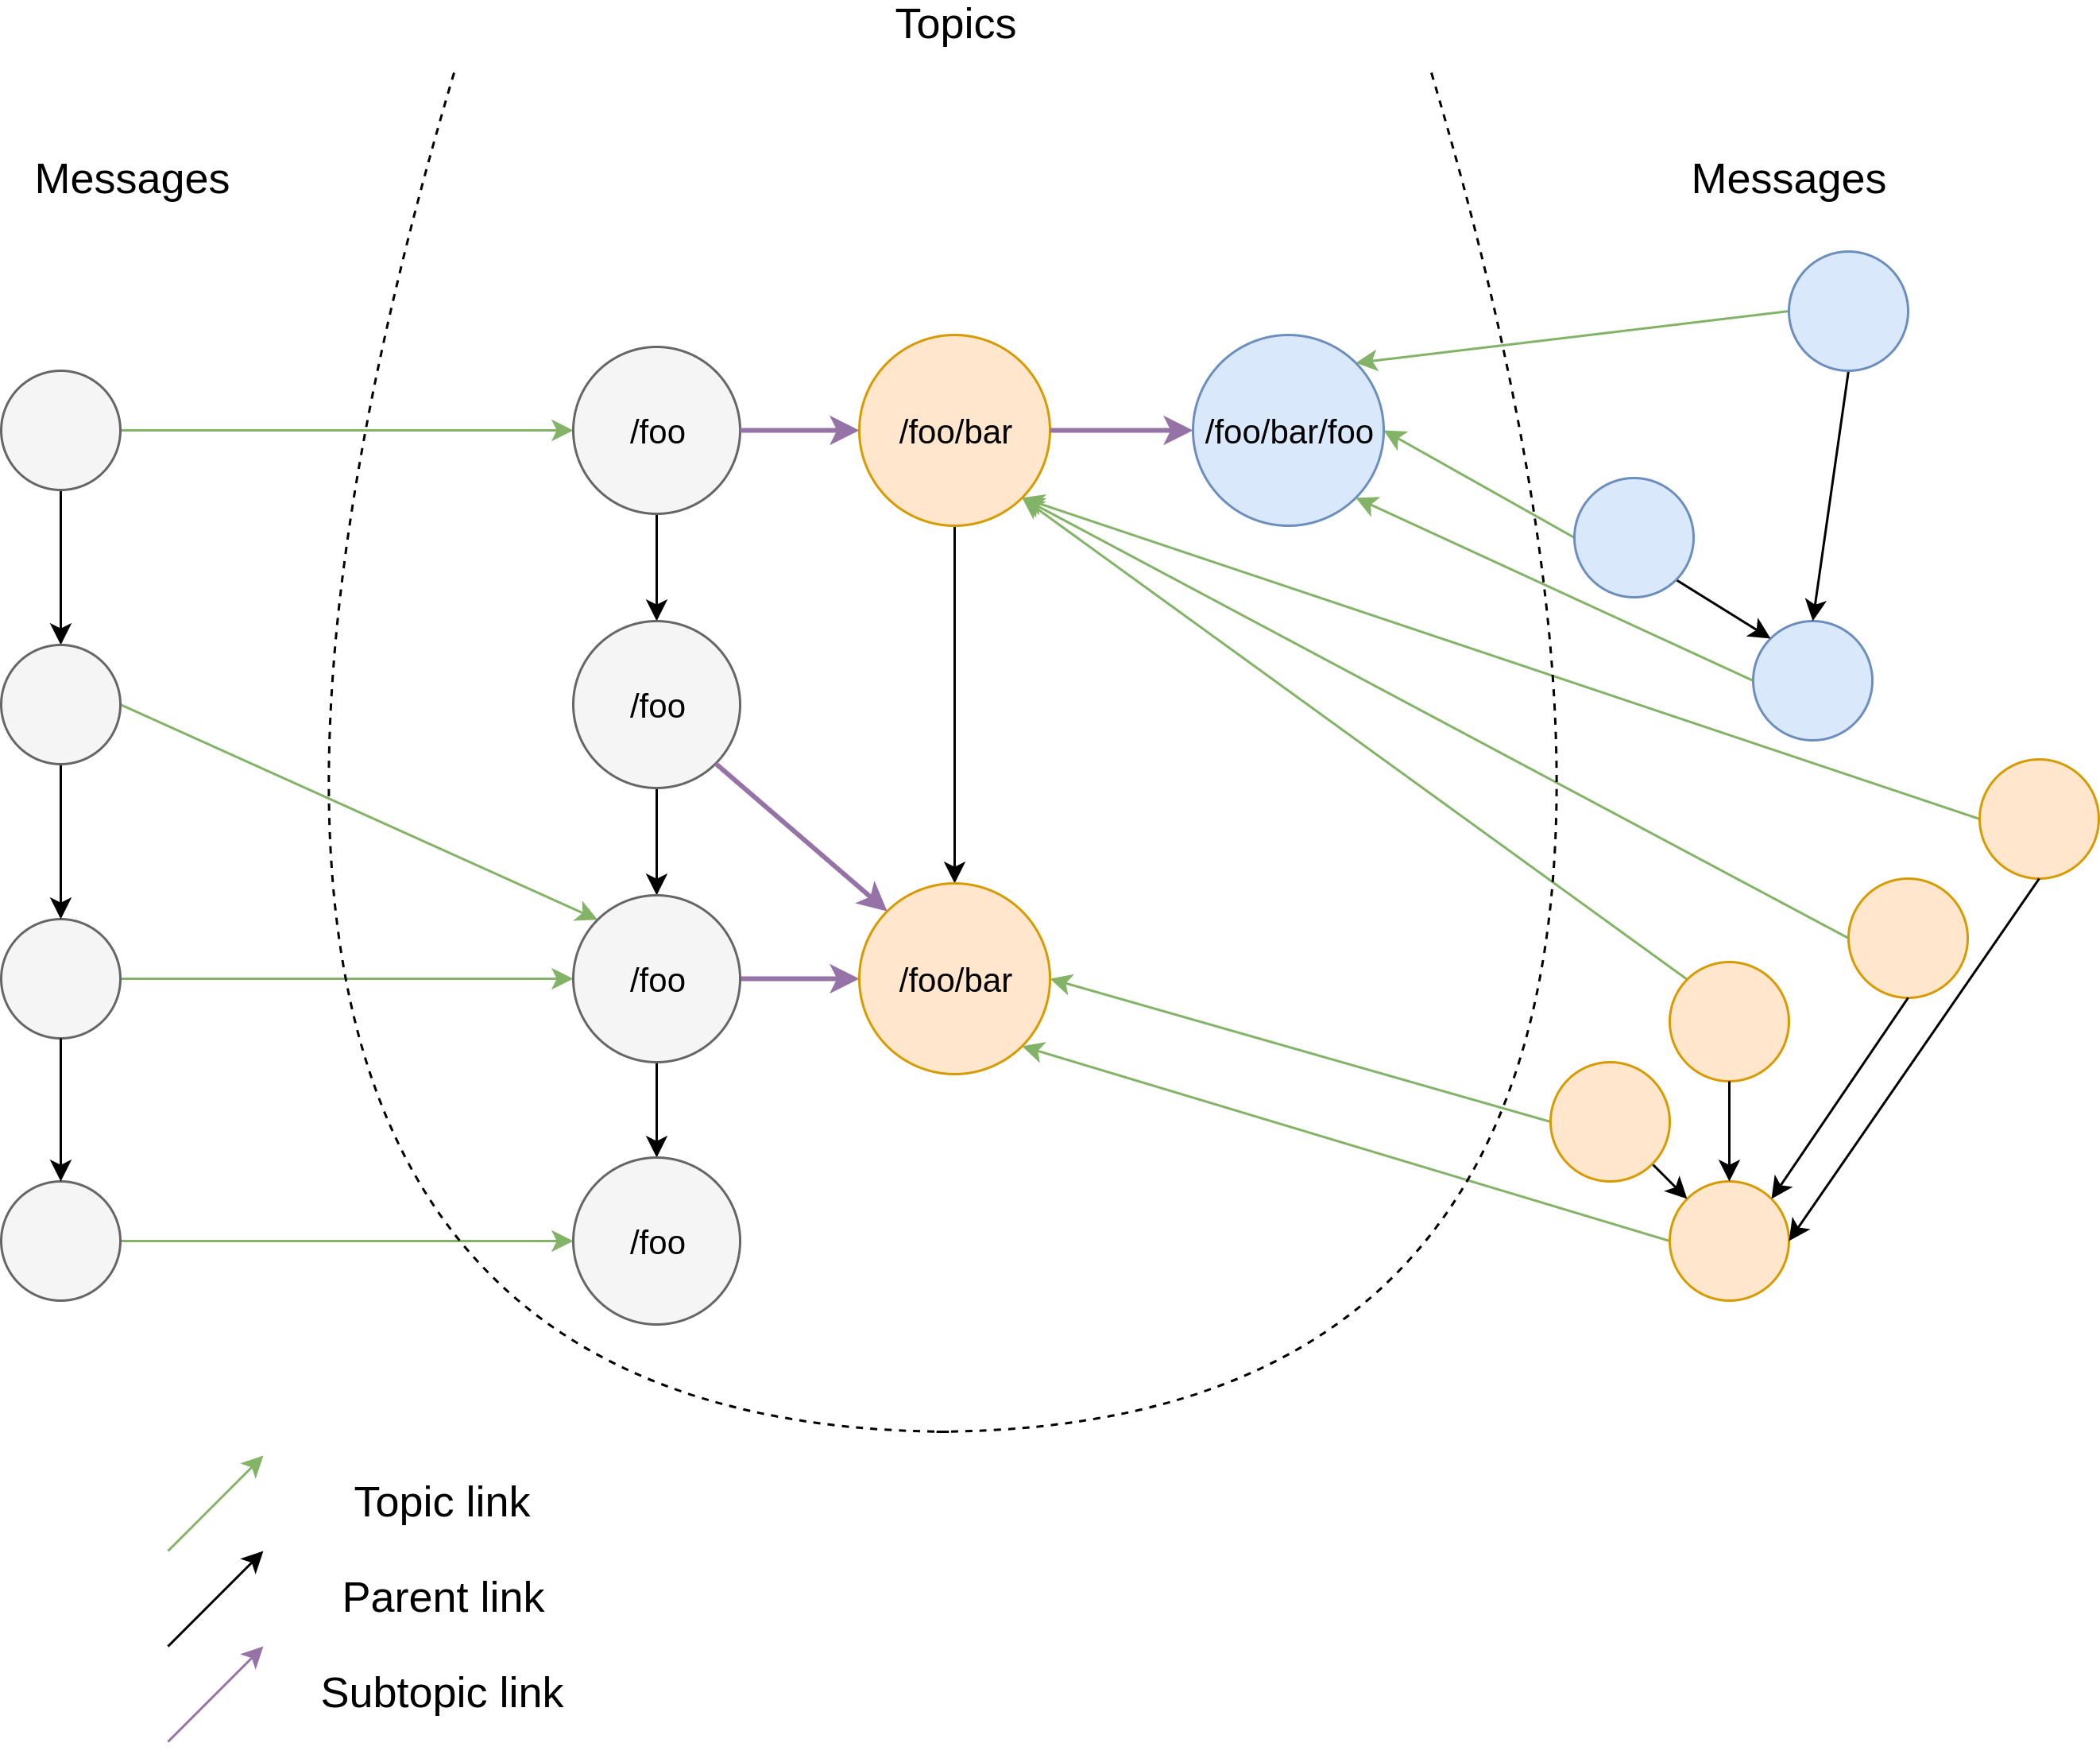
\includegraphics[width=0.95\textwidth]{img/pulsarcast-dag.png}
  \caption{Representation of the Pulsarcast DAG}
  \label{fig:pulsarcast-dag}
\end{figure}

\begin{figure}[hb!]
  \centering
  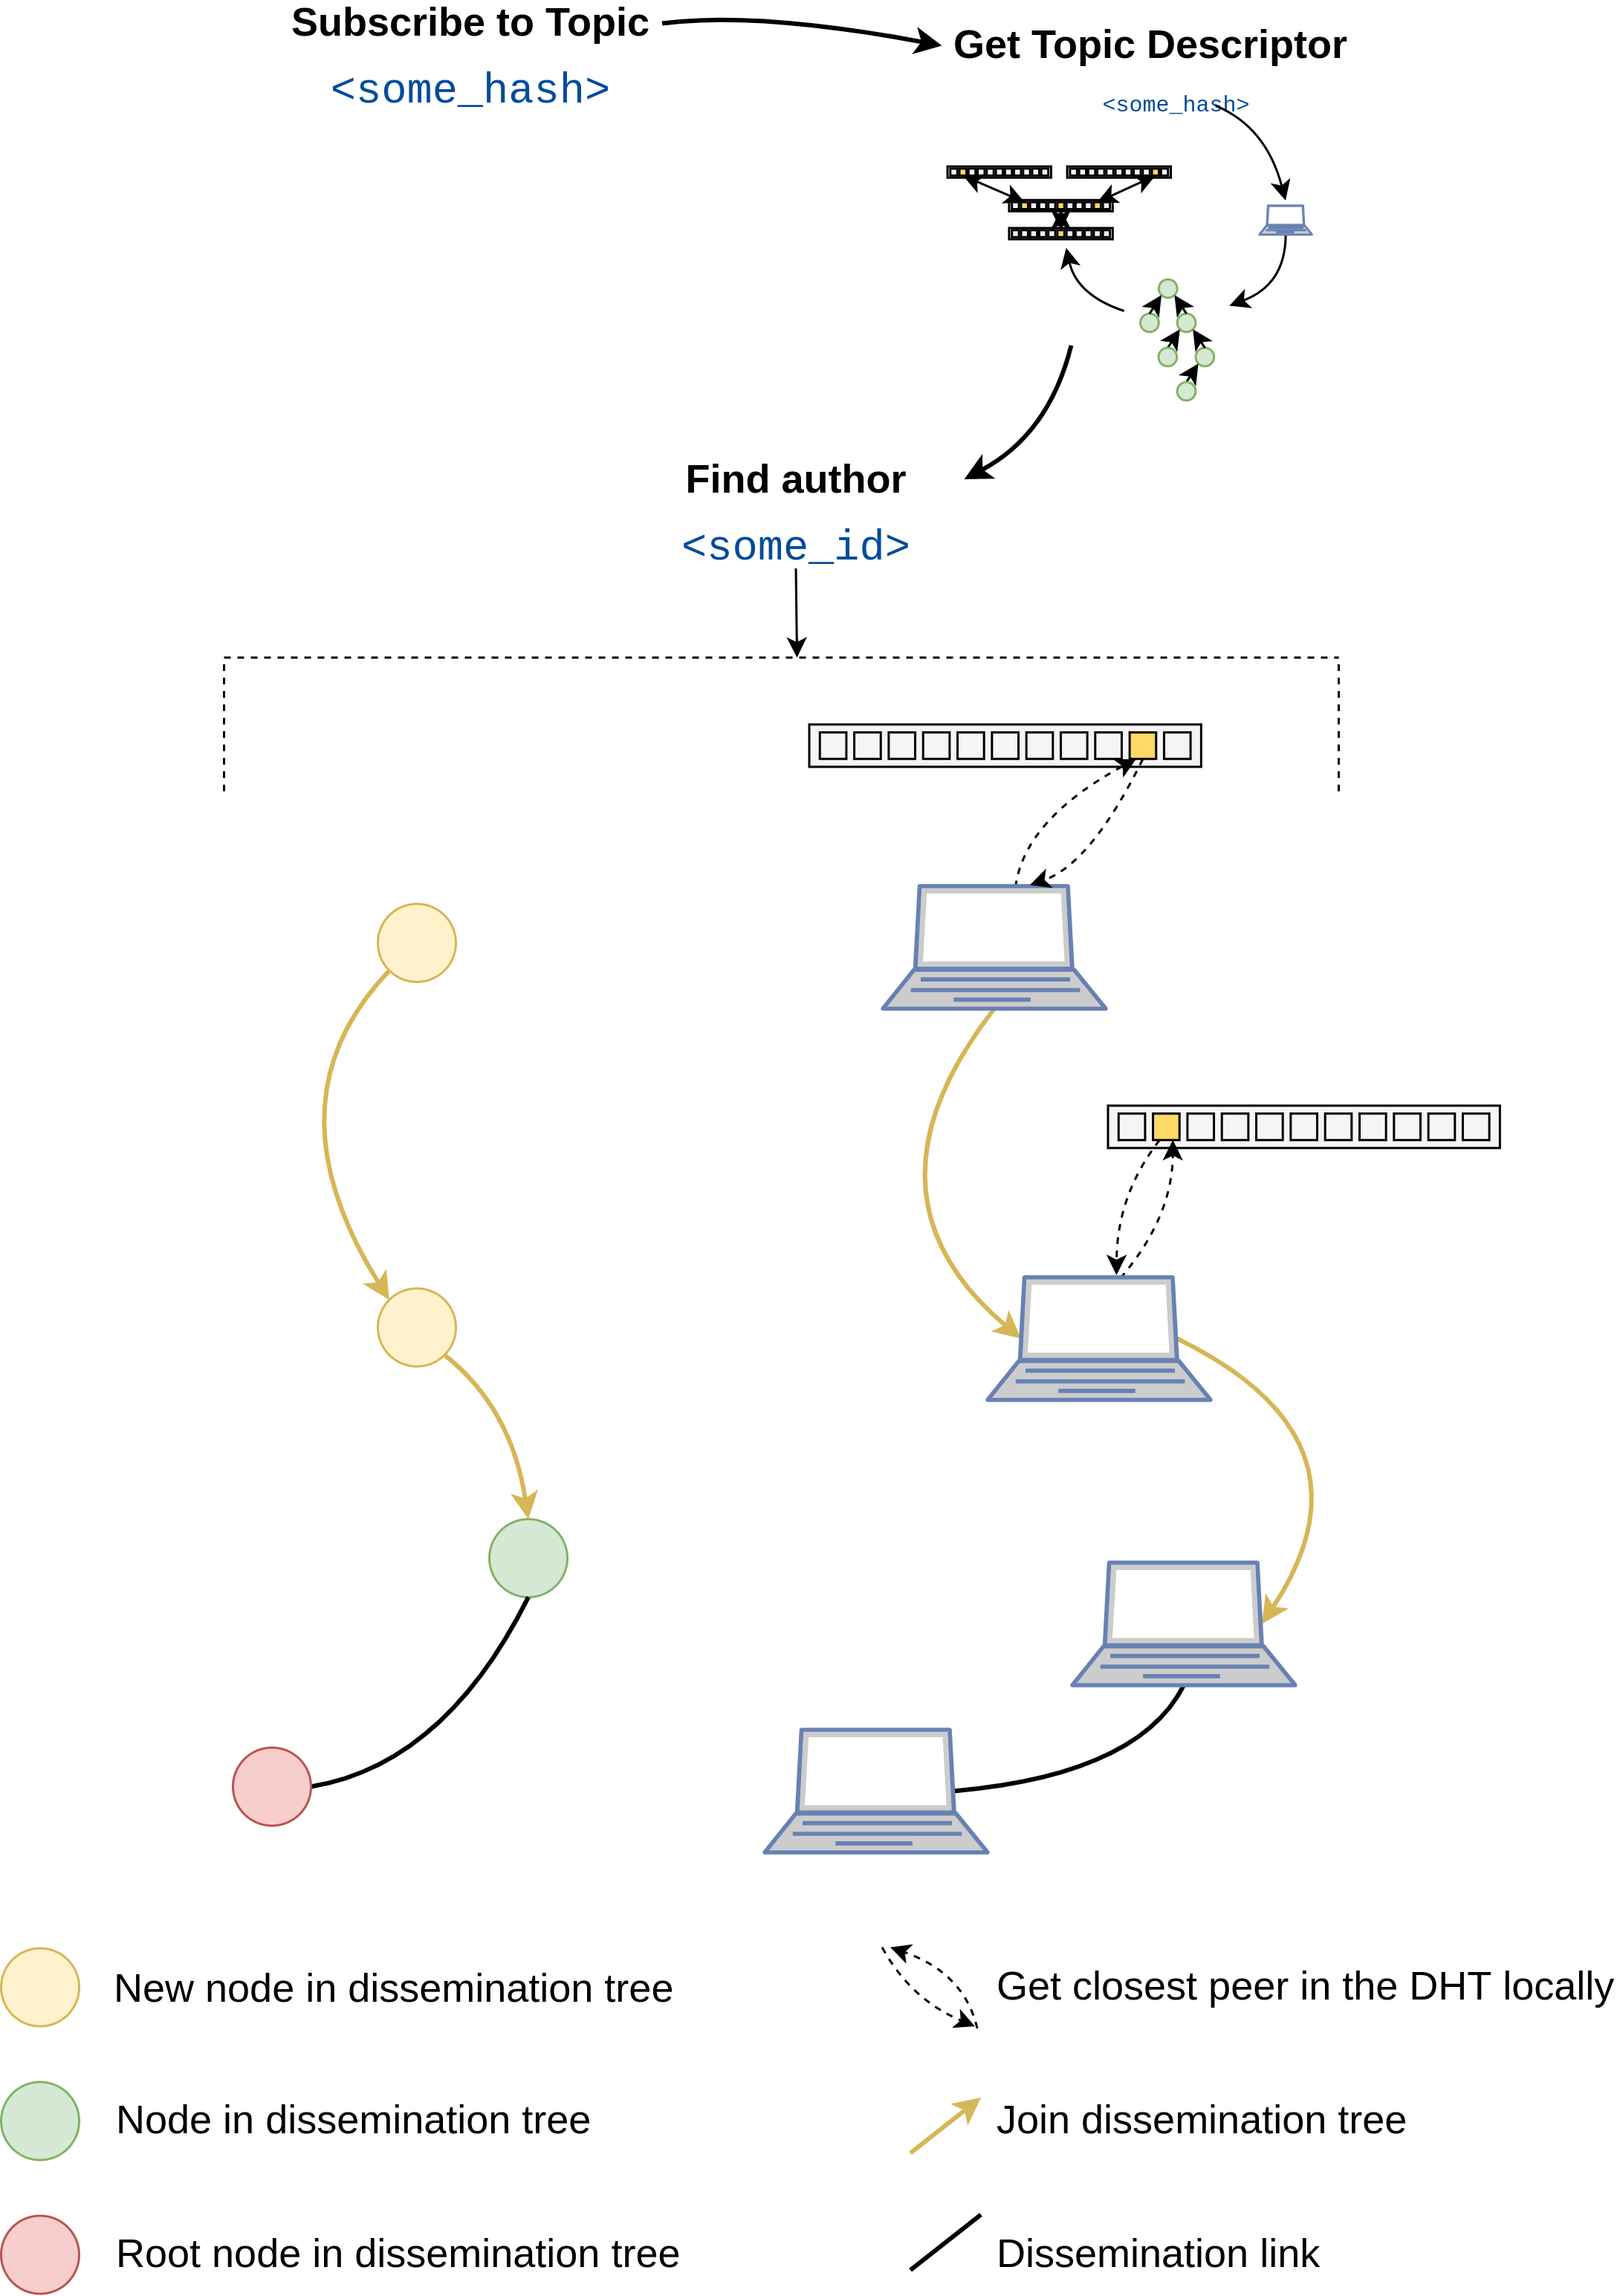
\includegraphics[width=0.95\textwidth]{img/pulsarcast-subscription-flow.png}
  \caption{Pulsarcast subscription flow}
  \label{fig:pulsarcast-subscription-flow}
\end{figure}

\SetKwProg{Fn}{Function}{}{}

\begin{algorithm}[H]
  \SetAlgoLined
  \Fn{CreateTopic(newTopic)}{
  	\KwIn{$newTopic=$ data for new topic creation}
		\BlankLine
  	\Begin{
			$parent \leftarrow newTopic.parent$\;
  	  \eIf(\tcp*[r]{Check if the topic has a parent link}){$parent == null$}{
				$metaTopic \leftarrow CreateMetaTopicDescriptor(newTopic)$\;
  	  }{
				$metaTopic \leftarrow parent.subTopics.meta$\;
			}
			$topicData \leftarrow CreateTopicDescriptor(newTopic, metaTopic)$\;
			$Subscribe(metaTopic)$\;
			$Subscribe(topicData)$\;
			$StoreInDHT(metaTopic)$\;
			$StoreInDHT(topicData)$\;
			$Publish(metaTopic, topicData)$\tcp*[r]{Publish the new topic in the meta topic}\
  	}
	}
  \caption{Create a new topic}
\end{algorithm}

TODO

\begin{algorithm}[H]
  \SetAlgoLined
  \Fn{ReceivedJoin(fromNodeId, topicId)}{
  	\KwData{$nodeId=$ node id of this node}
  	\KwIn{$topicId=$ topic id}
  	\KwIn{$fromNodeId=$ node who we got the join request from}
		\BlankLine
  	\Begin{
  	  $topicData \leftarrow GetTopicData(topicId)$\;
  	  \eIf{$fromNodeId \neq nodeId$}{
        $AddToChildren(t, fromNodeId)$\tcp*[r]{Add as children in dissemination tree}\
				\If(\tcp*[r]{This node is author of the topic}){$topicData.author == nodeId$}{
					\Return
				}
				\If(\tcp*[r]{Already part of dissemination tree}){$GetParents(topicId) \neq null$}{
					\Return
				}
  	  }{
				\If(\tcp*[r]{This node is author of the topic}){$topicData.author == nodeId$}{
					\Return
				}
			}
  	  $peer \leftarrow GetClosestKnownPeer(topicData.author)$\;
      $AddToParents(topicData.id, peer)$\tcp*[r]{Add as parent in dissemination tree}\
			$SendRPC(topicData.id, peer)$\;
  	}
	}
  \caption{Join request handler for each node}
\end{algorithm}

TODO

\begin{algorithm}[H]
  \SetAlgoLined
  \Fn{ReceivedEvent(fromNodeId, eventData)}{
  	\KwData{$nodeId=$ node id of this node}
  	\KwIn{$fromNodeId=$ node who we got the event from}
  	\KwIn{$eventData=$ event descriptor}
		\BlankLine
  	\Begin{
  	  $topicData \leftarrow GetTopicData(eventData.topicId)$\;
  	  \eIf{$AllowedToPublish(nodeId, topicData)$}{
				$SendEvent(fromNodeId, eventData)$\;
  	  }{
				\If{$AllowedToRequestToPublish(nodeId, topicData$}{
					$SendRequestToPublish(eventData)$\;
				}
			}
  	}
	}
  \caption{Event handler for each node}
\end{algorithm}

TODO

\begin{algorithm}[H]
  \SetAlgoLined
  \Fn{SendEvent(eventData)}{
  	\KwData{$nodeId=$ node id of this node}
  	\KwIn{$fromNodeId=$ node who we got the event from}
  	\KwIn{$eventData=$ event descriptor}
		\BlankLine
  	\Begin{
  	  $topicData \leftarrow GetTopicData(eventData.topicId)$\;
			\If{$IsNewEvent(eventData)$} {
				$linkedEvent \leftarrow LinkEvent(eventData)$\tcp*[r]{Add parent link}\
				$StoreInDHT(linkedEvent)$\;
			}
			\If{$(IsSubscribed(eventData.topicId)==true)$} {
				$EmitEvent(eventData.topicId, eventData)$\;
			}
			\For{$peer \leftarrow GetChildren(eventData.topicId), GetParents(eventData.topicId)$}{
				\If(\tcp*[r]{Don't send the event back}){$fromNodeId \neq peer$}{
					$SendRPC(eventData, peer)$\;
				}
			}
  	}
	}
  \caption{Event forwarding function}
\end{algorithm}


\section{RPC Protocol}
